% !TEX program = xelatex
\documentclass[12pt,a4paper]{article}

\usepackage{fontspec}
\usepackage{polyglossia}
\setmainlanguage{greek}
\setotherlanguage{english}
\setmainfont[Script=Greek]{DejaVu Serif}
\setsansfont[Script=Greek]{DejaVu Sans}
\setmonofont[Script=Greek]{DejaVu Sans Mono}
\newfontfamily\greekfonttt[Script=Greek]{DejaVu Sans Mono}

\usepackage[a4paper, margin=2.4cm]{geometry}
\usepackage{amsmath, amssymb}
\usepackage{booktabs}
\usepackage{array}
\usepackage{graphicx}
\usepackage{float}
\usepackage{caption}
\usepackage[hidelinks]{hyperref}
\usepackage{enumitem}
\usepackage{parskip}
\usepackage{xcolor}
\usepackage{fancyhdr}

\pagestyle{fancy}
\fancyhf{}
\lhead{Τεχνικές και Οργάνωση Ελέγχου Ποιότητας}
\rhead{Εργασία 2025--2026}
\cfoot{\thepage}
\setlength{\headheight}{14.5pt}

\captionsetup{font=small, labelfont=bf}
\graphicspath{{./}}
\renewcommand{\arraystretch}{1.18}
\setlength{\parindent}{0pt}
\sloppy

\newcommand{\code}[1]{\texttt{\textenglish{#1}}}
\newcommand{\Pa}{P_{\!a}}
\newcommand{\AOQ}{\textenglish{AOQ}}
\newcommand{\AOQL}{\textenglish{AOQL}}
\newcommand{\ATI}{\textenglish{ATI}}
\newcommand{\ASN}{\textenglish{ASN}}

\title{
    \textbf{Τεχνικές και Οργάνωση Ελέγχου Ποιότητας}\\[0.25cm]
    \Large Εργασία 2025--2026\\[0.15cm]
    \large Δειγματοληπτικός έλεγχος αποδοχής και διαγράμματα ελέγχου
}
\author{Τσακιρίδης}
\date{\today}

\begin{document}

\maketitle
\thispagestyle{fancy}

\begin{abstract}
Στην εργασία μελετώνται δύο βασικά θέματα ελέγχου ποιότητας. Στο πρώτο μέρος
προσδιορίζονται απλό και διπλό σχήμα δειγματοληπτικού ελέγχου αποδοχής με
διαλογή, με περιορισμούς ως προς τους κινδύνους παραγωγού και πελάτη και ως
προς το όριο μέσης εξερχόμενης ποιότητας. Στο δεύτερο μέρος κατασκευάζονται
διαγράμματα ελέγχου μέσης τιμής και τυπικής απόκλισης για την τάση εξόδου
τροφοδοτικών. Οι αριθμητικοί υπολογισμοί έγιναν με Python και τα αποτελέσματα
παρουσιάζονται αναλυτικά στους πίνακες και στα διαγράμματα που ακολουθούν.
\end{abstract}

\tableofcontents
\newpage

%=============================================================================
\section{Δεδομένα και υπολογιστική προσέγγιση}
%=============================================================================

Τα δεδομένα της εργασίας βρίσκονται στα αρχεία \code{parameters.csv} και
\code{data.csv}. Οι βασικές παράμετροι είναι οι εξής.

\begin{table}[H]
\centering
\caption{Παράμετροι του Μέρους Α.}
\begin{tabular}{lrl}
\toprule
\textbf{Παράμετρος} & \textbf{Τιμή} & \textbf{Περιγραφή} \\
\midrule
\(N\) & 600 & Μέγεθος παρτίδας \\
\(c_i\) & 6 & Κόστος ελέγχου ανά εξάρτημα \\
\(c_d\) & 400 & Κόστος ελαττωματικού που διαφεύγει \\
\(p_1\) & 0,0065 & Αποδεκτή στάθμη ποιότητας, ΑΣΠ \\
\(\alpha\) & 0,03 & Κίνδυνος παραγωγού \\
\(\beta\) & 0,10 & Κίνδυνος πελάτη \\
\(p_2=7p_1\) & 0,0455 & Μη αποδεκτή στάθμη ποιότητας \\
\(p_L,p_U\) & 0,004 και 0,060 & Όρια ομοιόμορφης κατανομής του \(p\) \\
\bottomrule
\end{tabular}
\end{table}

\begin{table}[H]
\centering
\caption{Παράμετροι του Μέρους Β.}
\begin{tabular}{lrl}
\toprule
\textbf{Παράμετρος} & \textbf{Τιμή} & \textbf{Περιγραφή} \\
\midrule
\(\mu_0\) & 9 V & Επιθυμητή μέση τάση \\
\(A\) & 0,10 V & Ημιπλάτος ορίων προδιαγραφών \\
\(\sigma\) & 0,035 V & Τυπική απόκλιση εντός ελέγχου \\
\(K\) & 21 & Κόστος κακής ποιότητας ανά ελαττωματικό \\
\(\Delta\) & 0,06 V & Μετατόπιση μέσης τιμής \\
\(k\) & 2,5 & Πλάτος ορίων ελέγχου σε τυπικές αποκλίσεις \\
\(n\) & 5 & Μέγεθος δείγματος ανά ώρα \\
\bottomrule
\end{tabular}
\end{table}

Για τον δειγματοληπτικό έλεγχο αποδοχής χρησιμοποιήθηκε το διωνυμικό μοντέλο
για τον αριθμό ελαττωματικών στο δείγμα. Με τον τρόπο αυτό η πιθανότητα
αποδοχής εκφράζεται ως συνάρτηση του ποσοστού ελαττωματικών \(p\). Όλα τα
αποτελέσματα αναπαράγονται από το αρχείο \code{toep\_solution.py}.

\newpage

%=============================================================================
\section{Μέρος Α: Δειγματοληπτικός έλεγχος αποδοχής}
%=============================================================================

\subsection{Απλό δειγματοληπτικό σχήμα}

Για απλό σχήμα \((n,c)\), η παρτίδα γίνεται αποδεκτή όταν ο αριθμός
ελαττωματικών στο δείγμα είναι το πολύ \(c\). Η χαρακτηριστική συνάρτηση
αποδοχής είναι:
\[
    \Pa(p)=\sum_{x=0}^{c}\binom{n}{x}p^x(1-p)^{n-x}.
\]

Οι περιορισμοί της εκφώνησης είναι:
\[
    \Pa(p_1)\ge 1-\alpha = 0{,}97,
    \qquad
    \Pa(p_2)\le \beta = 0{,}10.
\]

Επειδή γίνεται δειγματοληπτικός έλεγχος με διαλογή, όταν μια παρτίδα
απορρίπτεται ελέγχεται 100\%. Για απλό σχήμα έχουμε:
\[
    \AOQ(p)=p\,\Pa(p)\frac{N-n}{N},
\]
\[
    \ATI(p)=n+(N-n)\left[1-\Pa(p)\right].
\]

Ο επιπλέον περιορισμός είναι:
\[
    \AOQL \le 3p_1 = 0{,}0195.
\]

Ως καταλληλότερο σχήμα επιλέχθηκε το εφικτό σχήμα με το μικρότερο μέγεθος
δείγματος. Το αποτέλεσμα είναι:
\[
    \boxed{n=145,\qquad c=3}.
\]

\begin{table}[H]
\centering
\caption{Έλεγχος περιορισμών για το απλό σχήμα.}
\begin{tabular}{lr}
\toprule
\textbf{Μέγεθος} & \textbf{Τιμή} \\
\midrule
\(\Pa(p_1)\) & 0,98470 \\
\(1-\Pa(p_1)\) & 0,01530 \\
\(\Pa(p_2)\) & 0,09993 \\
\(\AOQL\) & 0,01016 \\
\(p\) στο οποίο εμφανίζεται το \(\AOQL\) & 0,02021 \\
\(\ATI(p_1)\) & 151,96 \\
\(\ATI(p_2)\) & 554,53 \\
\bottomrule
\end{tabular}
\end{table}

Το σχήμα ικανοποιεί και τους δύο κινδύνους, αφού ο κίνδυνος παραγωγού είναι
μικρότερος από 0,03 και ο κίνδυνος πελάτη είναι μικρότερος από 0,10. Επίσης,
το \(\AOQL=0{,}01016\) είναι αρκετά μικρότερο από το όριο \(0{,}0195\).

\subsection{Διπλό δειγματοληπτικό σχήμα}

Στο διπλό σχήμα δίνεται ότι \(c_1=0\), \(n_1=n_2\) και \(n_1+n_2>145\). Θέτουμε
\(n_1=n_2=m\). Η διαδικασία είναι:
\begin{itemize}[nosep]
    \item αποδοχή μετά το πρώτο δείγμα αν \(d_1=0\),
    \item απόρριψη μετά το πρώτο δείγμα αν \(d_1>c_2\),
    \item λήψη δεύτερου δείγματος αν \(1\le d_1\le c_2\),
    \item τελική αποδοχή αν \(d_1+d_2\le c_2\).
\end{itemize}

Η πιθανότητα αποδοχής γράφεται:
\[
    \Pa(p)=P_{a,1}(p)+P_{a,2}(p),
\]
όπου:
\[
    P_{a,1}(p)=P(D_1=0),
\]
\[
    P_{a,2}(p)=\sum_{d_1=1}^{c_2}P(D_1=d_1)\,
    P(D_2\le c_2-d_1).
\]

Για το διπλό σχήμα χρησιμοποιήθηκαν επίσης:
\[
    \ASN(p)=m+m\,P(1\le D_1\le c_2),
\]
\[
    \ATI(p)=mP_{a,1}(p)+2mP_{a,2}(p)+N\left[1-\Pa(p)\right].
\]

Με τους περιορισμούς της εκφώνησης προκύπτει:
\[
    \boxed{n_1=n_2=75,\qquad c_1=0,\qquad c_2=3}.
\]

\begin{table}[H]
\centering
\caption{Έλεγχος περιορισμών για το διπλό σχήμα.}
\begin{tabular}{lr}
\toprule
\textbf{Μέγεθος} & \textbf{Τιμή} \\
\midrule
\(\Pa(p_1)\) & 0,98381 \\
\(1-\Pa(p_1)\) & 0,01619 \\
\(\Pa(p_2)\) & 0,09990 \\
\(\AOQL\) & 0,01047 \\
\(p\) στο οποίο εμφανίζεται το \(\AOQL\) & 0,01975 \\
\(\ASN(p_1)\) & 103,90 \\
\(\ASN(p_2)\) & 114,23 \\
\(\ATI(p_1)\) & 111,30 \\
\(\ATI(p_2)\) & 552,76 \\
\bottomrule
\end{tabular}
\end{table}

Το διπλό σχήμα έχει συνολικό μέγιστο δείγμα \(150\), άρα ικανοποιεί τον
περιορισμό \(n_1+n_2>145\). Παράλληλα, διατηρεί τους απαιτούμενους κινδύνους
και έχει \(\AOQL=0{,}01047<0{,}0195\).

\subsection{Χαρακτηριστικές καμπύλες και μέσος αριθμός ελέγχων}

Στο Σχήμα~\ref{fig:oc-curves} φαίνονται οι χαρακτηριστικές καμπύλες των δύο
σχημάτων. Οι δύο καμπύλες είναι πολύ κοντά μεταξύ τους, κάτι αναμενόμενο,
επειδή και τα δύο σχήματα σχεδιάστηκαν ώστε να περνούν ουσιαστικά από τις
ίδιες απαιτήσεις στα σημεία \(p_1\) και \(p_2\).

\begin{figure}[H]
\centering
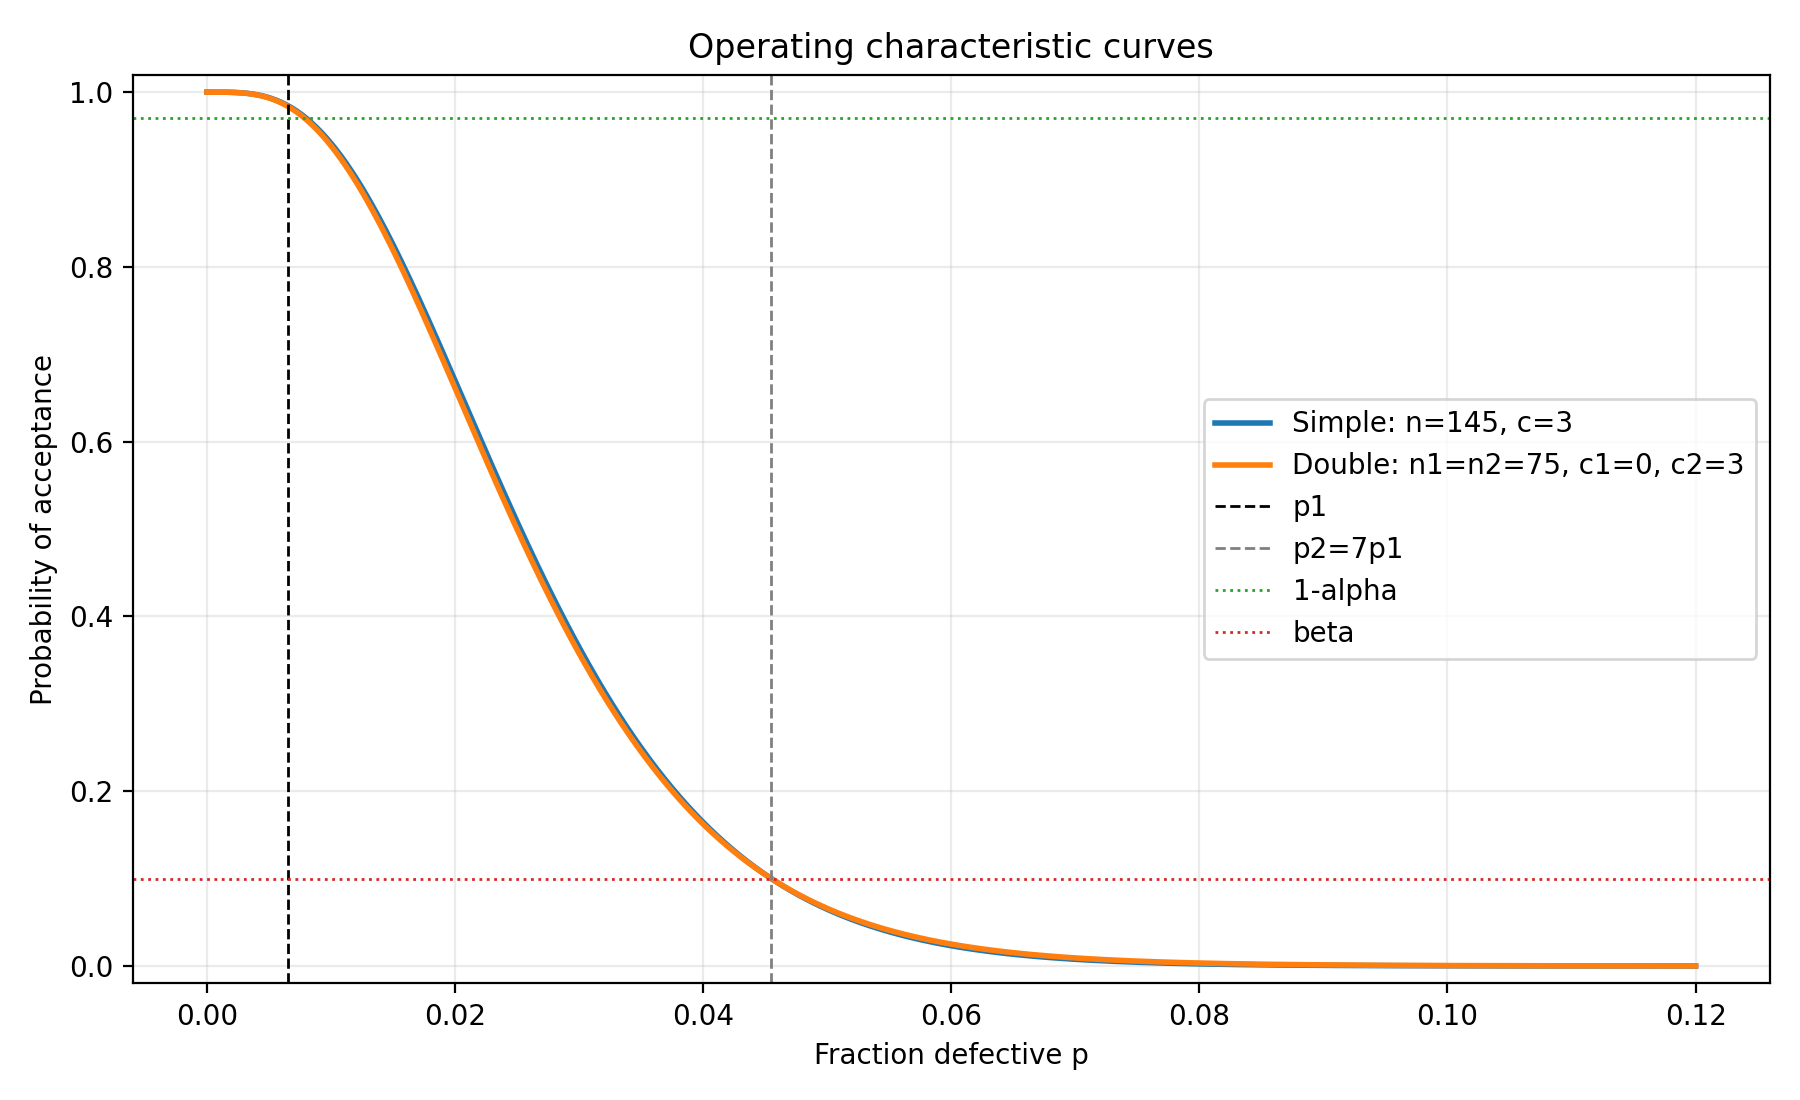
\includegraphics[width=0.92\textwidth]{acceptance_oc_curves.png}
\caption{Χαρακτηριστικές καμπύλες αποδοχής των δύο σχημάτων.}
\label{fig:oc-curves}
\end{figure}

Στο Σχήμα~\ref{fig:ati-curves} φαίνονται οι συναρτήσεις \(\ATI(p)\). Για πολύ
καλή ποιότητα, δηλαδή για μικρές τιμές του \(p\), το διπλό σχήμα έχει σαφώς
μικρότερο μέσο αριθμό επιθεωρούμενων μονάδων. Αυτό συμβαίνει επειδή πολλές
παρτίδες γίνονται αποδεκτές ήδη από το πρώτο δείγμα των 75 τεμαχίων. Αντίθετα,
στο απλό σχήμα ελέγχονται πάντοτε 145 τεμάχια πριν ληφθεί απόφαση.

Όταν το ποσοστό ελαττωματικών αυξάνεται, και τα δύο σχήματα οδηγούν συχνότερα
σε απόρριψη και συνεπώς σε πλήρη έλεγχο της παρτίδας. Για αυτό οι καμπύλες
\(\ATI(p)\) πλησιάζουν το \(N=600\).

\begin{figure}[H]
\centering
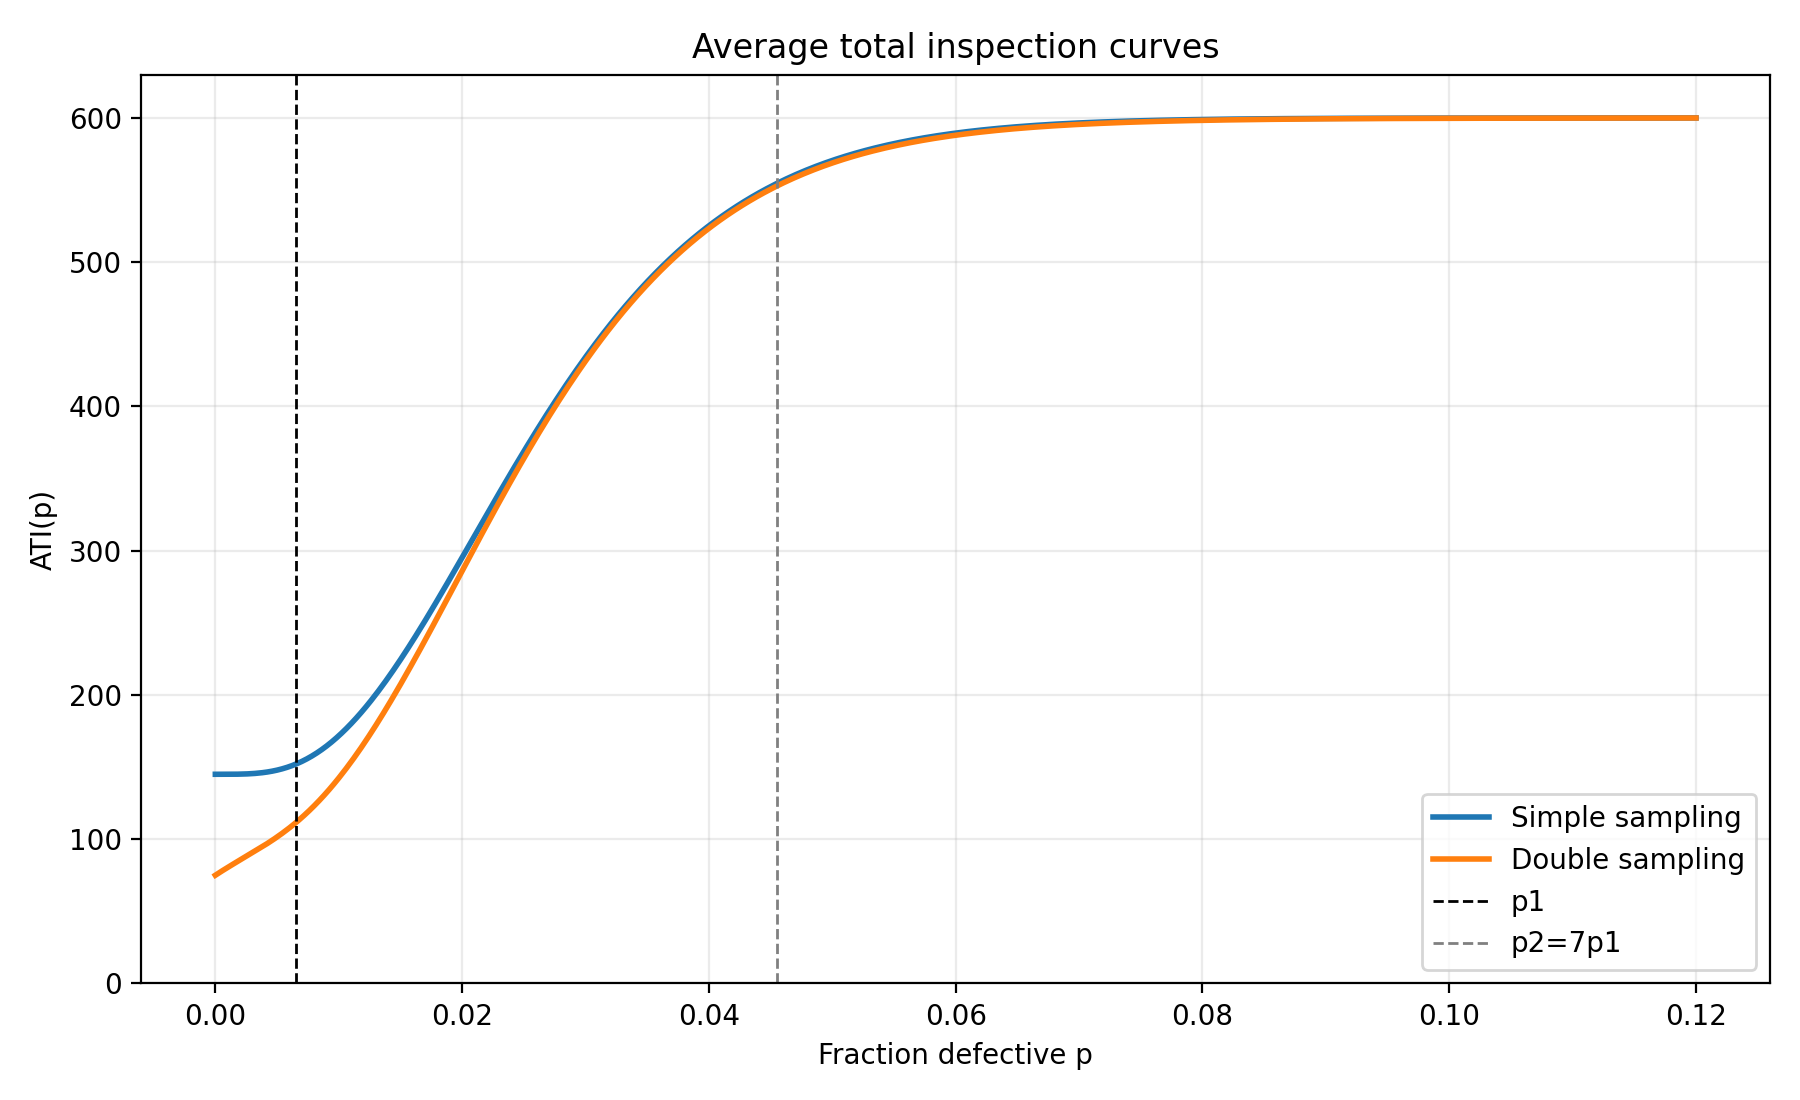
\includegraphics[width=0.92\textwidth]{acceptance_ati_curves.png}
\caption{Μέσος συνολικός αριθμός επιθεωρούμενων μονάδων \(\ATI(p)\).}
\label{fig:ati-curves}
\end{figure}

Στο Σχήμα~\ref{fig:aoq-curves} παρουσιάζονται και οι καμπύλες \(\AOQ(p)\), ώστε
να φαίνεται γραφικά ότι και τα δύο σχήματα βρίσκονται κάτω από το επιτρεπτό
όριο \(3p_1\).

\begin{figure}[H]
\centering
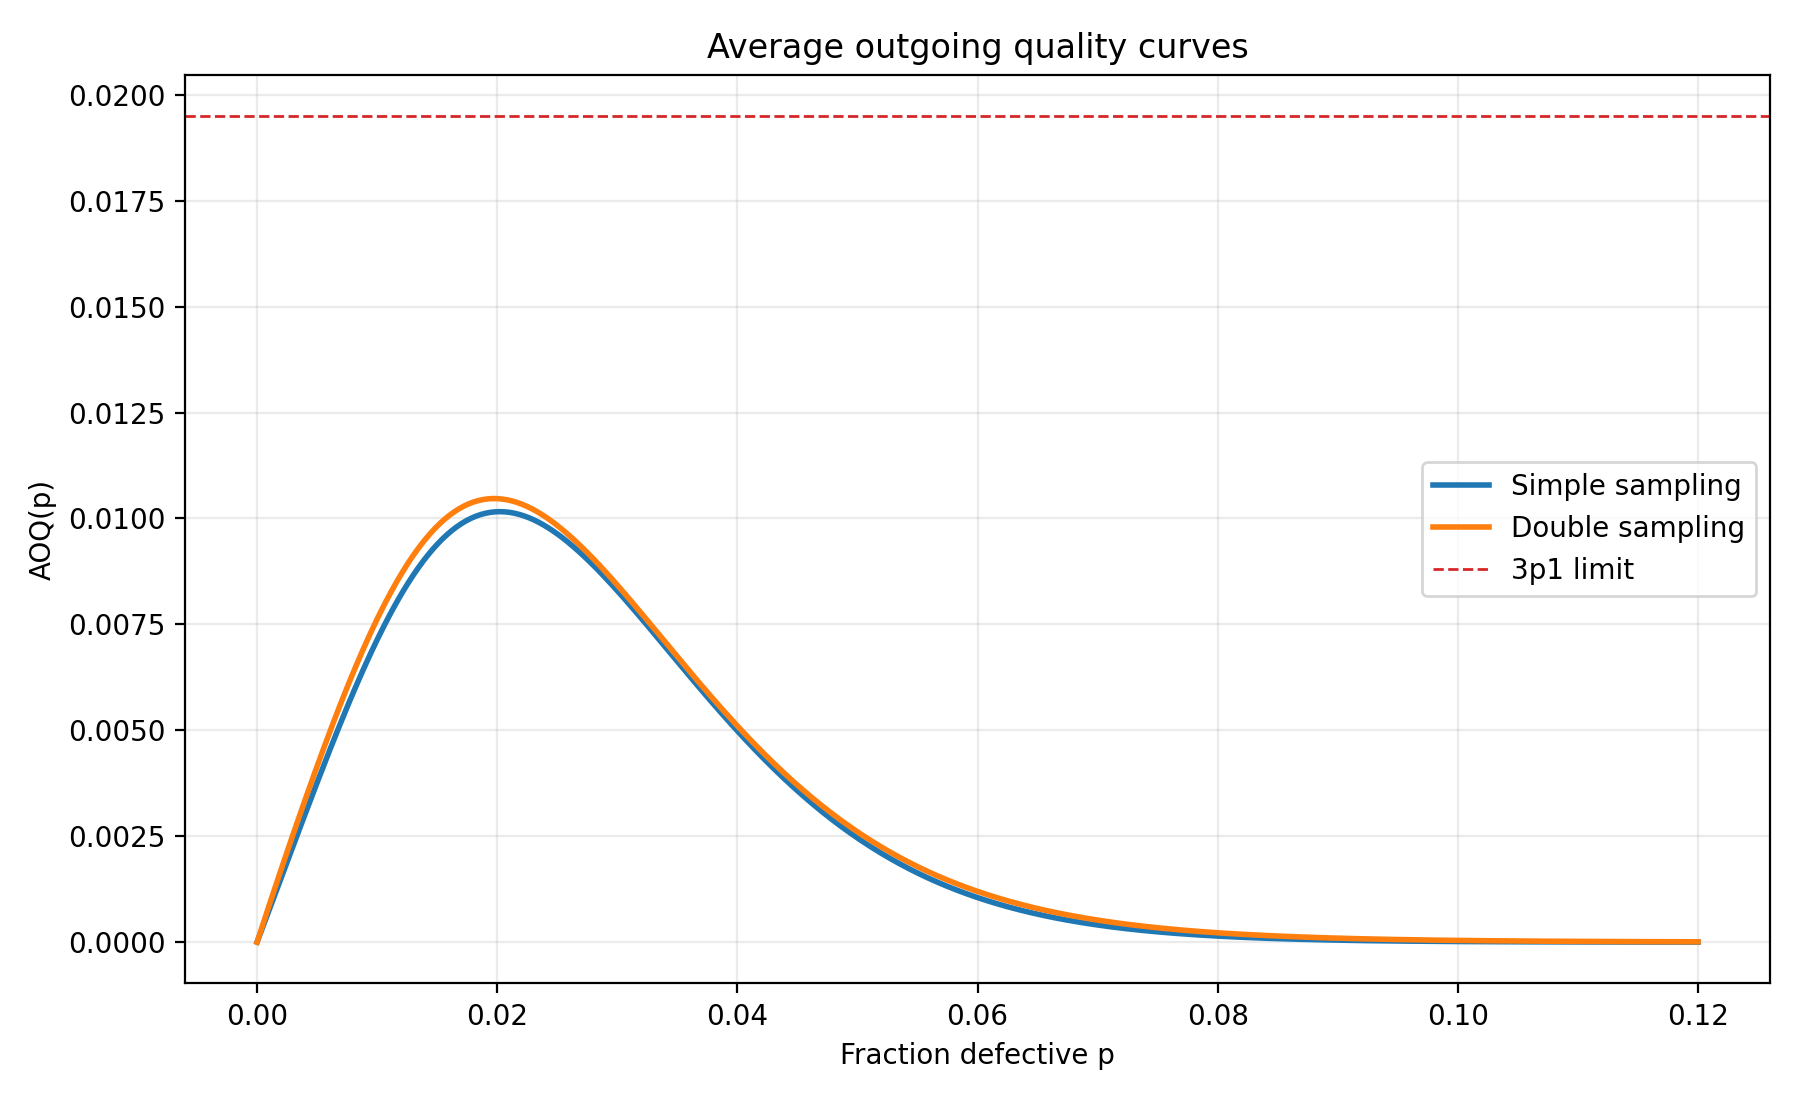
\includegraphics[width=0.92\textwidth]{acceptance_aoq_curves.png}
\caption{Μέση εξερχόμενη ποιότητα \(\AOQ(p)\) και όριο \(3p_1\).}
\label{fig:aoq-curves}
\end{figure}

\subsection{Βέλτιστο απλό σχήμα ως προς το κόστος}

Στο τελευταίο ερώτημα του Μέρους Α θεωρούμε ότι το πραγματικό ποσοστό
ελαττωματικών μιας παρτίδας ακολουθεί ομοιόμορφη κατανομή στο διάστημα:
\[
    p\sim U(0{,}004,\;0{,}060).
\]

Για απλό σχήμα \((n,c)\), το συνολικό κόστος ανά παρτίδα για συγκεκριμένο
ποσοστό ελαττωματικών \(p\) είναι:
\[
    C(p)=c_i\,\ATI(p)+c_d\,p\,\Pa(p)(N-n).
\]

Ο πρώτος όρος είναι το κόστος ελέγχου. Ο δεύτερος όρος είναι το κόστος των
ελαττωματικών που διαφεύγουν, δηλαδή των ελαττωματικών που βρίσκονται εκτός
του δείγματος σε παρτίδες που γίνονται αποδεκτές.

Το μέσο συνολικό κόστος είναι:
\[
    E[C]=\frac{1}{p_U-p_L}\int_{p_L}^{p_U} C(p)\,dp.
\]

Με περιορισμό \(c\le 1\), το βέλτιστο απλό σχήμα είναι:
\[
    \boxed{n=189,\qquad c=1}.
\]

\begin{table}[H]
\centering
\caption{Σύγκριση μέσου συνολικού κόστους.}
\begin{tabular}{lrrr}
\toprule
\textbf{Σχήμα} & \textbf{\(n\)} & \textbf{\(c\)} & \textbf{Μέσο κόστος ανά παρτίδα} \\
\midrule
Βέλτιστο με \(c\le 1\) & 189 & 1 & 3.522,36 € \\
Σχήμα Ερωτήματος Α1 & 145 & 3 & 3.912,03 € \\
\bottomrule
\end{tabular}
\end{table}

Το σχήμα του Ερωτήματος Α1 έχει μέσο κόστος μεγαλύτερο κατά:
\[
    3.912{,}03-3.522{,}36 = 389{,}67 \text{ € ανά παρτίδα}.
\]

Σε ποσοστιαία μορφή:
\[
    \frac{389{,}67}{3.522{,}36}\cdot 100 = 11{,}06\%.
\]

Άρα, αν το μοναδικό κριτήριο είναι το μέσο συνολικό κόστος και επιτρέπονται
μόνο απλά σχήματα με \(c\le 1\), το σχήμα \((189,1)\) είναι προτιμότερο από το
σχήμα του πρώτου ερωτήματος. Το σχήμα του Α1 όμως είχε σχεδιαστεί για να
ικανοποιεί συγκεκριμένους κινδύνους παραγωγού και πελάτη και τον περιορισμό
\(\AOQL\).

\newpage

%=============================================================================
\section{Μέρος Β: Διαγράμματα ελέγχου για τάση εξόδου}
%=============================================================================

\subsection{Όρια ελέγχου μέσης τιμής και τυπικής απόκλισης}

Η παραγωγική διαδικασία έχει επιθυμητή μέση τιμή \(\mu_0=9\) V και τυπική
απόκλιση \(\sigma=0{,}035\) V. Για δείγματα μεγέθους \(n=5\), το διάγραμμα
μέσης τιμής έχει όρια:
\[
    UCL_{\bar X}=\mu_0+k\frac{\sigma}{\sqrt{n}},
    \qquad
    CL_{\bar X}=\mu_0,
    \qquad
    LCL_{\bar X}=\mu_0-k\frac{\sigma}{\sqrt{n}}.
\]

Με \(k=2{,}5\):
\[
    LCL_{\bar X}=8{,}960869,\qquad
    CL_{\bar X}=9{,}000000,\qquad
    UCL_{\bar X}=9{,}039131.
\]

Για το διάγραμμα τυπικής απόκλισης χρησιμοποιείται:
\[
    E(S)=c_4\sigma,
    \qquad
    \sigma_S=\sigma\sqrt{1-c_4^2},
\]
όπου για \(n=5\):
\[
    c_4=\sqrt{\frac{2}{n-1}}\frac{\Gamma(n/2)}{\Gamma((n-1)/2)}
    =0{,}939986.
\]

Άρα:
\[
    UCL_S=c_4\sigma+k\sigma_S,
    \qquad
    CL_S=c_4\sigma,
    \qquad
    LCL_S=\max(0,c_4\sigma-k\sigma_S).
\]

Τα όρια είναι:
\[
    LCL_S=0{,}003043,\qquad
    CL_S=0{,}032899,\qquad
    UCL_S=0{,}062756.
\]

\begin{table}[H]
\centering
\caption{Όρια των διαγραμμάτων ελέγχου.}
\begin{tabular}{lrrr}
\toprule
\textbf{Διάγραμμα} & \textbf{LCL} & \textbf{CL} & \textbf{UCL} \\
\midrule
\(\bar X\) & 8,960869 & 9,000000 & 9,039131 \\
\(S\) & 0,003043 & 0,032899 & 0,062756 \\
\bottomrule
\end{tabular}
\end{table}

\subsection{Πιθανότητα σφάλματος πρώτου είδους}

Για το διάγραμμα μέσης τιμής, όταν η διαδικασία είναι εντός ελέγχου:
\[
    \alpha_{\bar X}=P(|Z|>2{,}5)=2[1-\Phi(2{,}5)].
\]

Άρα:
\[
    \alpha_{\bar X}=0{,}012419.
\]

Για το διάγραμμα \(S\) χρησιμοποιείται η ακριβής κατανομή:
\[
    \frac{(n-1)S^2}{\sigma^2}\sim \chi^2_{n-1}.
\]

Έτσι:
\[
    \alpha_S=0{,}012095.
\]

Επειδή για κανονική κατανομή η \(\bar X\) και το \(S\) είναι ανεξάρτητα, η
πιθανότητα εσφαλμένης ένδειξης από ένα τουλάχιστον διάγραμμα είναι:
\[
    \alpha_{\text{ολ}}=
    1-(1-\alpha_{\bar X})(1-\alpha_S).
\]

Άρα:
\[
    \boxed{\alpha_{\text{ολ}}=0{,}024364}.
\]

\subsection{Ισχύς του διαγράμματος μέσης τιμής}

Όταν η μέση τιμή μετατοπιστεί από \(9\) σε \(9\pm\Delta\), με
\(\Delta=0{,}06\), η ισχύς του διαγράμματος μέσης τιμής είναι η πιθανότητα η
\(\bar X\) να βρεθεί εκτός των ορίων ελέγχου.

Λόγω συμμετρίας, η ισχύς είναι ίδια για μετατόπιση προς τα πάνω και προς τα
κάτω. Τα αποτελέσματα είναι:

\begin{table}[H]
\centering
\caption{Ισχύς του διαγράμματος \(\bar X\).}
\begin{tabular}{lr}
\toprule
\textbf{Περίπτωση} & \textbf{Ισχύς} \\
\midrule
Μεταβολή μέσης τιμής, χωρίς μεταβολή \(\sigma\) & 0,908777 \\
Μεταβολή μέσης τιμής και αύξηση \(\sigma\) κατά 20\% & 0,866727 \\
\bottomrule
\end{tabular}
\end{table}

Η αύξηση της τυπικής απόκλισης μειώνει ελαφρά την ισχύ του διαγράμματος μέσης
τιμής στη συγκεκριμένη μετατόπιση, επειδή η κατανομή της \(\bar X\) γίνεται
πιο απλωμένη και μέρος της πιθανότητας μένει εντός των σταθερών ορίων ελέγχου.

\subsection{Ισχύς του διαγράμματος τυπικής απόκλισης}

Για αύξηση της τυπικής απόκλισης από \(\sigma\) σε \(1{,}2\sigma\), η ισχύς
του διαγράμματος \(S\) είναι:
\[
    P(S<LCL_S \ \text{ή}\ S>UCL_S \mid \sigma'=1{,}2\sigma).
\]

Το αποτέλεσμα είναι:
\[
    \boxed{0{,}062919}.
\]

Η ισχύς αυτή δεν επηρεάζεται από παράλληλη μεταβολή της μέσης τιμής, επειδή η
κατανομή του \(S\) για κανονικά δεδομένα εξαρτάται από την τυπική απόκλιση και
όχι από τη μέση τιμή. Συνεπώς:

\begin{table}[H]
\centering
\caption{Ισχύς του διαγράμματος \(S\).}
\begin{tabular}{lr}
\toprule
\textbf{Περίπτωση} & \textbf{Ισχύς} \\
\midrule
Αύξηση \(\sigma\) κατά 20\%, χωρίς μεταβολή μέσης τιμής & 0,062919 \\
Αύξηση \(\sigma\) κατά 20\%, με παράλληλη μεταβολή μέσης τιμής & 0,062919 \\
\bottomrule
\end{tabular}
\end{table}

\subsection{Μέσο κόστος κακής ποιότητας μέχρι την ανίχνευση}

Τα όρια προδιαγραφών είναι:
\[
    LSL=9-A=8{,}90,\qquad USL=9+A=9{,}10.
\]

Μετά τη μεταβολή της μέσης τιμής σε \(9+\Delta=9{,}06\) και με την τυπική
απόκλιση αμετάβλητη, η πιθανότητα να παραχθεί ελαττωματικό τροφοδοτικό είναι:
\[
    P(X<8{,}90)+P(X>9{,}10)=0{,}126551.
\]

Ο ρυθμός παραγωγής είναι 100 τροφοδοτικά ανά ώρα και το κόστος κακής ποιότητας
είναι 21 € ανά ελαττωματικό. Άρα το αναμενόμενο κόστος κακής ποιότητας ανά
ώρα μετά τη μετατόπιση είναι:
\[
    0{,}126551 \cdot 100 \cdot 21 = 265{,}76 \text{ €/ώρα}.
\]

Η πιθανότητα ανίχνευσης της μεταβολής από το διάγραμμα \(\bar X\) σε κάθε
δείγμα είναι η ισχύς:
\[
    \pi=0{,}908777.
\]

Επομένως ο μέσος αριθμός δειγμάτων μέχρι την ένδειξη είναι:
\[
    ARL_1=\frac{1}{\pi}=1{,}10038.
\]

Αν η μεταβολή συμβεί σε τυχαία στιγμή μέσα στο ωριαίο διάστημα μεταξύ δύο
δειγματοληψιών, ο μέσος χρόνος μέχρι την ανίχνευση είναι:
\[
    ATS=1\cdot\left(ARL_1-\frac{1}{2}\right)=0{,}60038 \text{ ώρες}.
\]

Άρα το μέσο κόστος κακής ποιότητας μέχρι την ανίχνευση είναι:
\[
    265{,}76\cdot 0{,}60038
    =
    \boxed{159{,}56 \text{ €}}.
\]

Αν, πιο συντηρητικά, θεωρήσουμε ότι η μεταβολή συμβαίνει αμέσως μετά από μια
δειγματοληψία, τότε ο μέσος χρόνος μέχρι την ένδειξη είναι \(1{,}10038\) ώρες
και το αντίστοιχο κόστος γίνεται:
\[
    265{,}76\cdot 1{,}10038 = 292{,}43 \text{ €}.
\]

\subsection{Έλεγχος των 15 δειγμάτων}

Με βάση τα 15 δείγματα υπολογίστηκαν η δειγματική μέση τιμή και η δειγματική
τυπική απόκλιση κάθε δείγματος. Τα αποτελέσματα παρουσιάζονται στον
Πίνακα~\ref{tab:samples}.

\begin{table}[H]
\centering
\caption{Αποτελέσματα ελέγχου για τα 15 δείγματα.}
\label{tab:samples}
\small
\begin{tabular}{rrrrl}
\toprule
\textbf{Δείγμα} & \textbf{\(\bar x\)} & \textbf{\(s\)} & \textbf{Εκτός \(\bar X\)} & \textbf{Συμπέρασμα} \\
\midrule
1 & 8,992 & 0,04087 & Όχι & Εντός ελέγχου \\
2 & 9,018 & 0,03033 & Όχι & Εντός ελέγχου \\
3 & 9,012 & 0,02775 & Όχι & Εντός ελέγχου \\
4 & 9,024 & 0,04506 & Όχι & Εντός ελέγχου \\
5 & 8,984 & 0,01140 & Όχι & Εντός ελέγχου \\
6 & 9,006 & 0,02302 & Όχι & Εντός ελέγχου \\
7 & 8,980 & 0,05148 & Όχι & Εντός ελέγχου \\
8 & 9,012 & 0,03271 & Όχι & Εντός ελέγχου \\
9 & 9,004 & 0,04930 & Όχι & Εντός ελέγχου \\
10 & 9,058 & 0,04087 & Ναι & Εκτός ελέγχου \\
11 & 9,086 & 0,03362 & Ναι & Εκτός ελέγχου \\
12 & 9,070 & 0,00707 & Ναι & Εκτός ελέγχου \\
13 & 9,038 & 0,04207 & Όχι & Εντός ελέγχου \\
14 & 9,066 & 0,03715 & Ναι & Εκτός ελέγχου \\
15 & 9,072 & 0,04147 & Ναι & Εκτός ελέγχου \\
\bottomrule
\end{tabular}
\end{table}

Κανένα από τα 15 δείγματα δεν είναι εκτός ελέγχου στο διάγραμμα \(S\). Όμως τα
δείγματα 10, 11, 12, 14 και 15 υπερβαίνουν το άνω όριο του διαγράμματος
\(\bar X\). Άρα η διαδικασία δεν μπορεί να θεωρηθεί ότι βρισκόταν σε
στατιστικό έλεγχο σε όλη τη διάρκεια λήψης των 15 δειγμάτων. Η ένδειξη είναι
κυρίως μετατόπιση της μέσης τάσης προς μεγαλύτερες τιμές, όχι αύξηση της
μεταβλητότητας.

\begin{figure}[H]
\centering
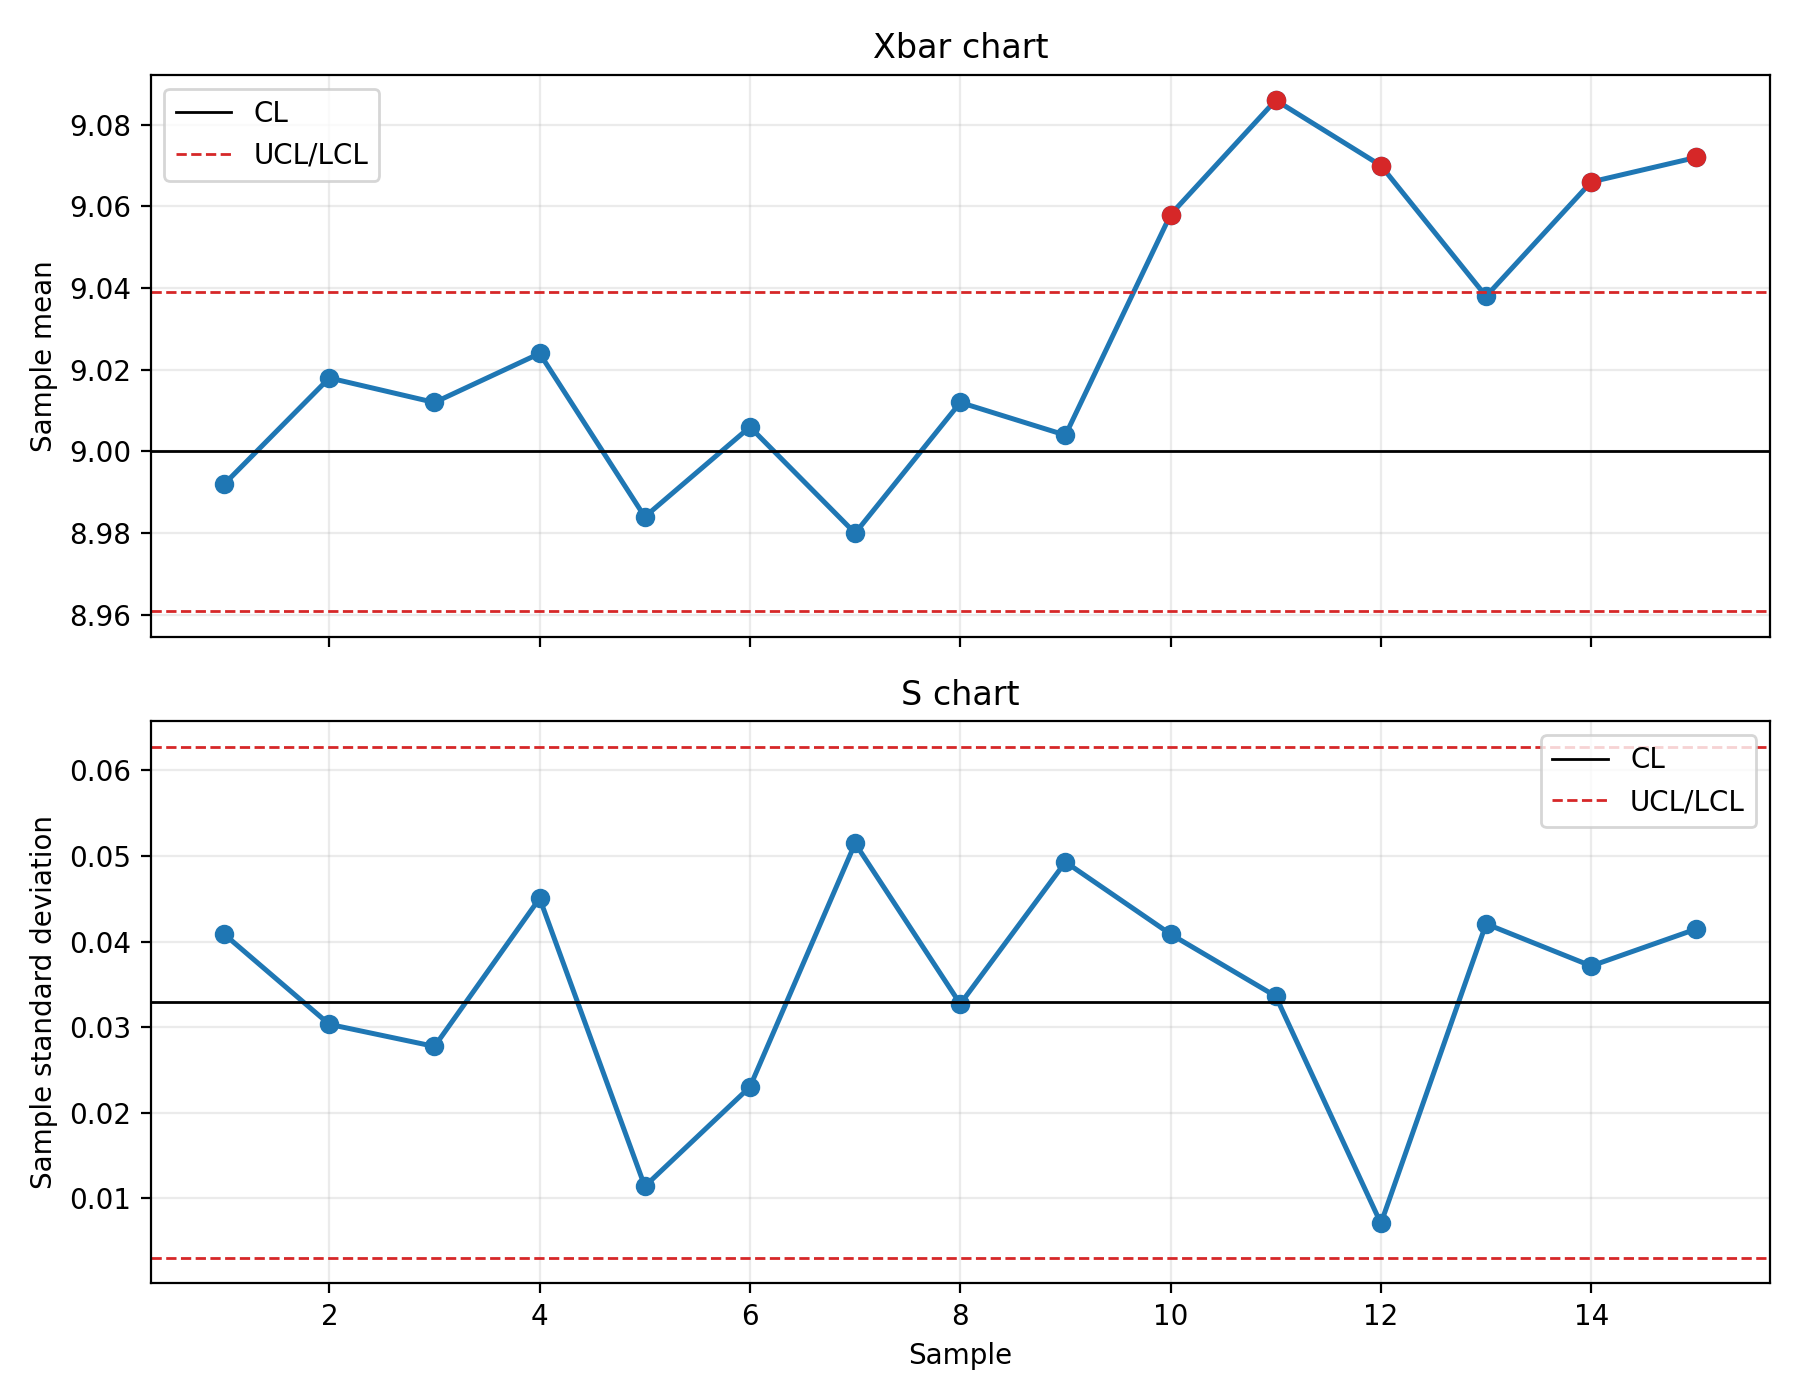
\includegraphics[width=0.92\textwidth]{control_charts_samples.png}
\caption{Διαγράμματα \(\bar X\) και \(S\) για τα 15 δείγματα.}
\label{fig:control-charts}
\end{figure}

%=============================================================================
\section{Συμπεράσματα}
%=============================================================================

Στο Μέρος Α, το απλό σχήμα που ικανοποιεί τους κινδύνους παραγωγού και πελάτη
και τον περιορισμό \(\AOQL\) είναι το \((n,c)=(145,3)\). Το αντίστοιχο διπλό
σχήμα με \(c_1=0\), ίσα δείγματα και \(n_1+n_2>145\) είναι
\((n_1,n_2,c_1,c_2)=(75,75,0,3)\). Το διπλό σχήμα έχει παρόμοια
χαρακτηριστική καμπύλη, αλλά μικρότερο μέσο αριθμό επιθεωρούμενων μονάδων όταν
η ποιότητα είναι καλή.

Στο κριτήριο μέσου κόστους, με \(c\le 1\), το καλύτερο απλό σχήμα είναι
\((189,1)\), με μέσο κόστος 3.522,36 € ανά παρτίδα. Το σχήμα του πρώτου
ερωτήματος έχει μέσο κόστος 3.912,03 € ανά παρτίδα, δηλαδή είναι ακριβότερο
κατά 11,06\%.

Στο Μέρος Β, τα διαγράμματα ελέγχου έχουν όρια
\(\bar X\): 8,960869 έως 9,039131 και \(S\): 0,003043 έως 0,062756. Η συνολική
πιθανότητα εσφαλμένης ένδειξης από ένα τουλάχιστον διάγραμμα είναι 0,024364.
Στα πραγματικά δείγματα εμφανίζονται εκτός ελέγχου τα δείγματα 10, 11, 12, 14
και 15 από το διάγραμμα \(\bar X\), ενώ το διάγραμμα \(S\) δεν δίνει ένδειξη
εκτός ελέγχου.

\end{document}
